% METODOLOGIA------------------------------------------------------------------

\chapter{METODOLOGIA}
\label{chap:metodologia}
Neste capítulo são descritas as etapas do desenvolvimento desta monografia, sendo elas a formulação e pré-processamento da base de dados, a configuração da rede neural e sua codificação utilizando o \textit{framework} \textit{keras} \cite{chollet2015keras}, além de pesquisas e aplicações de melhorias para a rede neural proposta, como o \textit{data augmentation} e a inicialização dos pesos a partir de valores de uma rede já treinada.

\section{Formulação da base}
No aprendizado de máquina, é recomendável que a base de dados em que foram feitos os treinos e os testes do método escolhido possua balanceamento na distribuição de amostras por classes, e as amostras de uma mesma classe precisam ter características que as diferenciem das outras amostras de outras classes.

\par Neste trabalho foi feita a classificação de imagens de comida, dessa maneira, a base montada contém amostras segregadas em classes como \textit{pizza} e \textit{sushi}. Também foram adicionadas classes de imagens que não estão relacionadas com comida, como \textit{plant}(no português, planta) e \textit{domestic animals}(no português, animais domésticos), visando melhorar o classificador, quando utilizado em bases que possuam imagens não associadas à comida.
\par As imagens selecionadas para a formulação do conjunto de dados deste trabalho foram retiradas das bases de dados \textit{ImageNet}\cite{deng2009imagenet} e \textit{Food-101}\cite{bossard14}. A base \textit{ImageNet} é densamente estruturada e organizada em hierarquia de árvore, facilitando assim encontrar as categorias que estão relacionadas ao tema abordado. Já a base \textit{Food-101} é composta de 101 classes de imagens de comida, selecionadas e com um tamanho fixo de 1000 imagens por classe. A precisão de categorização das bases \textit{ImageNet} e \textit{Food-101} são necessárias para a formulação da base de teste deste projeto, tendo em vista que a categorização manual de imagens não seria uma abordagem viável, uma vez que redes neurais convolucionais demandam uma grande quantidade de imagens para um treinamento adequado.  

\par A base formulada possui um total de $16000$ imagens separadas em 16 classes, sendo dessas classes 13 relacionadas com comida (\textit{chocolate cake, french fries, hamburger, ice cream, pizza, spaghetti bolognese, sushi,club sandwich, filet mignon, fried rice, hot dog, steak, tacos}) e três não relacionadas com comida (\textit{domestic animal, people, plant}). Como descrito na \autoref{tab:base_images}, é possível identificar que as imagens das 13 classes relacionadas com comida foram retiradas da base de dados \textit{Food-101}, elas foram selecionadas com base na popularidade dos tipos de comida que representam, como \textit{pizza} e macarrão (\textit{spaghetti bolognese}). As imagens das três classes restantes foram retiradas da base de dados \textit{ImageNet}, foram escolhidas visando abranger imagens que possam ocorrer em bases de dados que não sejam só de comidas, buscando melhorar o desempenho das classificações nessas bases. Na \autoref{fig:imagebase} podemos ver um exemplo da diversidade dessas imagens.
\begin{figure}[H]
  \centering
  \caption{Exemplos de imagens encontradas na base de dados.}
  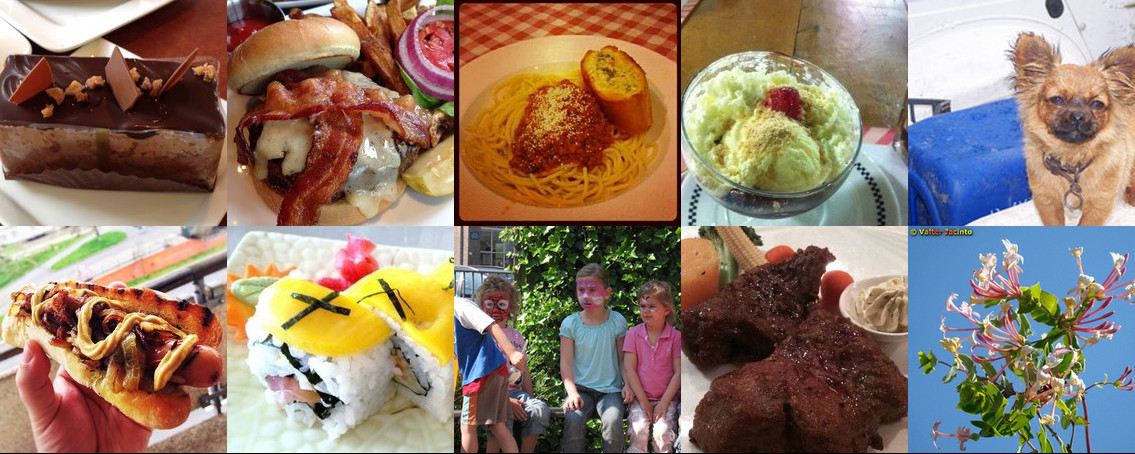
\includegraphics[width=300pt]{dados/figuras/imagembase}
  \fonte{imagens retiradas das bases \textit{ImageNet}\cite{deng2009imagenet} e \textit{Food-101}\cite{bossard14}}
  \label{fig:imagebase}
\end{figure}

\subsection{Pré-processamento}
\par Redes neurais convolucionais requerem uma grande quantidade de imagens. Dessa maneira, as entradas fornecidas para a rede neural devem seguir um padrão, sendo que todas as imagens precisam possuir as mesmas dimensões. Assim as imagens foram redimensionadas para $227\times227$ \textit{pixels}, tendo em vista que é um valor que proporcionou bons resultados em trabalhos semelhantes \cite{imaginetArticle}. Nas alterações de dimensões das imagens foi realizado um corte nas imagens originais para forçar uma formato quadrado antes de ser aplicado o redimensionamento, preservando os formatos das imagens. As perdas de informações que podem ocorrer com os cortes realizados nas imagens são pequenas, sabendo que os objetos relevantes para a classificação estão apresentados no centro e os cortes são realizados nas extremidades das imagens. Com o uso da função de \textit{max pooling} possíveis perdas de informações relevantes que podem ocorrer nos cortes das imagens são reparadas.  

\par Para a realização dos treinos e testes com a rede neural, a base de dados foi separada em dados de treino e de teste. Como informado na \autoref{tab:base_images}, 70\% das imagens (11200 imagens) de cada classe foram utilizadas para o treino da rede neural, e os 30\% das imagens restantes (4800 imagens) foram utilizadas para a fase de teste da rede neural.

\begin{table}[H]
    \centering
    \caption[Disposição da base de dados]{Separação da base de dados em classes, sendo informada a quantidade de amostras separadas para realizar as etapas de treino e teste, também é informado a base de origem do dado.
    \label{tab:base_images}}
    \begin{tabular}{ccccc}
        \toprule
             Classe & Amostras de treino & Amostras de teste & Amostras totais & Base de origem \\
        \midrule
            chocolate cake & 700 & 300 & 1000 & \textit{Food-101}\\
            french fries & 700 & 300 & 1000 & \textit{Food-101}\\
            hamburger & 700 & 300 & 1000 & \textit{Food-101}\\
            ice cream & 700 & 300 & 1000 & \textit{Food-101}\\
            pizza & 700 & 300 & 1000 & \textit{Food-101}\\
            spaghetti bolognese & 700 & 300 & 1000 & \textit{Food-101}\\
            sushi & 700 & 300 & 1000 & \textit{Food-101}\\
            club sandwich & 700 & 300 & 1000 & \textit{Food-101}\\
            filet mignon & 700 & 300 & 1000 & \textit{Food-101}\\
            fried rice & 700 & 300 & 1000 & \textit{Food-101}\\
            hot dog & 700 & 300 & 1000 & \textit{Food-101}\\
            steak & 700 & 300 & 1000 & \textit{Food-101}\\
            tacos & 700 & 300 & 1000 & \textit{Food-101}\\
            domestic animal & 700 & 300 & 1000 & \textit{ImageNet}\\
            people & 700 & 300 & 1000 & \textit{ImageNet}\\
            plant & 700 & 300 & 1000 & \textit{ImageNet}\\

        \bottomrule
    \end{tabular}
\end{table}



\section{Configuração da Rede Neural}

A configuração da rede neural convolucional utilizada neste projeto é fundamentada na rede neural \textit{AlexNet} definida por \citeonline{imaginetArticle}. A \textit{AlexNet} é uma rede neural convolucional que foi proposta para solucionar o problema do desafio LSVRC de 2012 promovido pela equipe da \textit{Image-Net}\footnote{http://image-net.org/challenges/LSVRC/2012/index, acessado em 04 de janeiro de 2018.}. Ela obteve grande destaque ao conseguir realizar a classificação de 1.2 milhões de imagens em 1000 classes, obtendo o melhor resultado do desafio utilizando o \textit{Top-5}, apresentando uma taxa de erro de 15,3\%, muito superior ao segundo colocado, que apresentou uma taxa de erro de 26,2\%. A estrutura da \textit{AlexNet} é composta por cinco camadas convolucionais, na qual algumas são seguidas por uma camada de \textit{max pooling}, e três camadas fortemente conectadas, em que a última apresenta 1.000 neurônios de saída e aplica a função de ativação \textit{softmax}. Outro destaque apresentado pela \textit{AlexNet} foi o emprego do método de \textit{dropout} nas camadas fortemente conectadas, com o intuito de reduzir o \textit{overfitting}.

\par A rede neural proposta neste projeto utiliza de oito camadas ocultas de processamento, sendo cinco camadas convolucionais e três camadas fortemente conectadas. Tendo em vista que a rede escolhida como exemplo foi estruturada para classificar mil classes, foi necessário fazer algumas adaptações para classificar uma quantidade menor de classes. Uma dessas alterações foi a modificação da função \textit{softmax} para obter o resultado da classificação na última camada conforme descrito na \autoref{fig:arqrede}. A função de ativação ReLu foi usada em todas as camadas da rede, exceto na camada de saída, em que foi aplicada a função \textit{softmax}.

\par A primeira camada de convolução da rede separa a entrada, uma imagem de $227\times227\times3$ em 96 núcleos de $11\times11\times3$ (com uma distância de 4 \textit{pixels} entre os centros das imagens vizinhas), em que cada imagem gerada é processada separadamente. 
Gerando uma imagem $55\times55\times96$, na qual $55\times55$ representa as dimensões da imagem e 96 a quantidade de filtros que foram gerados nela. Após essa camada, é aplicada uma camada de \textit{max pooling} em regiões de $3\times3$ \textit{pixels} da imagem, com uma distância de $2\times2$ \textit{pixels} entre os centros da regiões, resultando em uma imagem de $27\times27\times96$.

\par A segunda camada convolucional tem como entrada a saída da primeira camada convolucional normalizada e com \textit{pooling} aplicado. Essa entrada tem o formato de $27\times27\times96$ é filtrada em 256 núcleos de $5\times5\times96$, gerando uma saída de $27\times27\times256$ com as mesmas dimensões aumentado a quantidade de filtros aplicados. Após essa camada também é aplicada uma camada de \textit{max pooling} com as mesmas configurações da camada de \textit{max pooling} anterior, resultando em uma saída de $13\times13\times256$.

\par A terceira camada convolucional possui 384 núcleos de $3\times3\times256$ que são conectados à entrada fornecida pela saída da segunda camada convolucional normalizada e aplicado o \textit{pooling}. O formato da saída gerada pela terceira camada é de $13\times13\times384$. As conexões entre a terceira, quarta e quinta camada convolucional não possuem nenhuma operação de \textit{pooling} entre si. 

\par Assim, a quarta camada convolucional possui 384 núcleos de $3\times3\times384$ e gera uma saída de formato $13\times13\times384$, na qual só é aplicada a convolução e não é modificada a entrada.

\par A quinta camada possui 256 núcleos de $3\times3\times384$ e gera uma saída com o formato de $13\times13\times256$, reduzindo a quantidades de filtros aplicados na imagem. Após a quinta camada convolucional é aplicada uma camada de \textit{max pooling} com as mesmas configurações das outras camadas de \textit{max pooling} utilizadas na rede, gerando uma saída de $6\times6\times256$.

\par As duas camadas seguintes são camadas fortemente conectadas com 4096 neurônios cada, com no fim de cada uma aplicada a função de \textit{dropout} inicialmente com uma taxa de 50\%. A função de ativação das camadas fortemente conectadas foi o ReLu. Por fim uma camada com 16 neurônios (um neurônio para cada classe) fortemente conectada com a operação de \textit{softmax} para obter a predição da entrada. O processo de aprendizagem utilizados nas camadas fortemente conectadas foi o \textit{backpropagation}. A taxa de aprendizagem utilizada durante o \textit{backpropagation} foi de $0,01\%$, tendo em vista que foram obtidos bons resultados utilizando esse valor em outras redes neurais convolucionais \cite{imaginetArticle}.

\begin{figure}[H]
  \centering
  \caption{Diagrama que representa a arquitetura da rede neural convolucional proposta. O formato de cada camada da rede é descrito na seta que incide nele, e o formato que ele gera é infomado na seta que sai dele. Como exemplo a operação de convolução da camada convolucional 1, na qual a sua entrada é de $227\times227\times3$ e sua saída é de $55\times55\times96$.}
  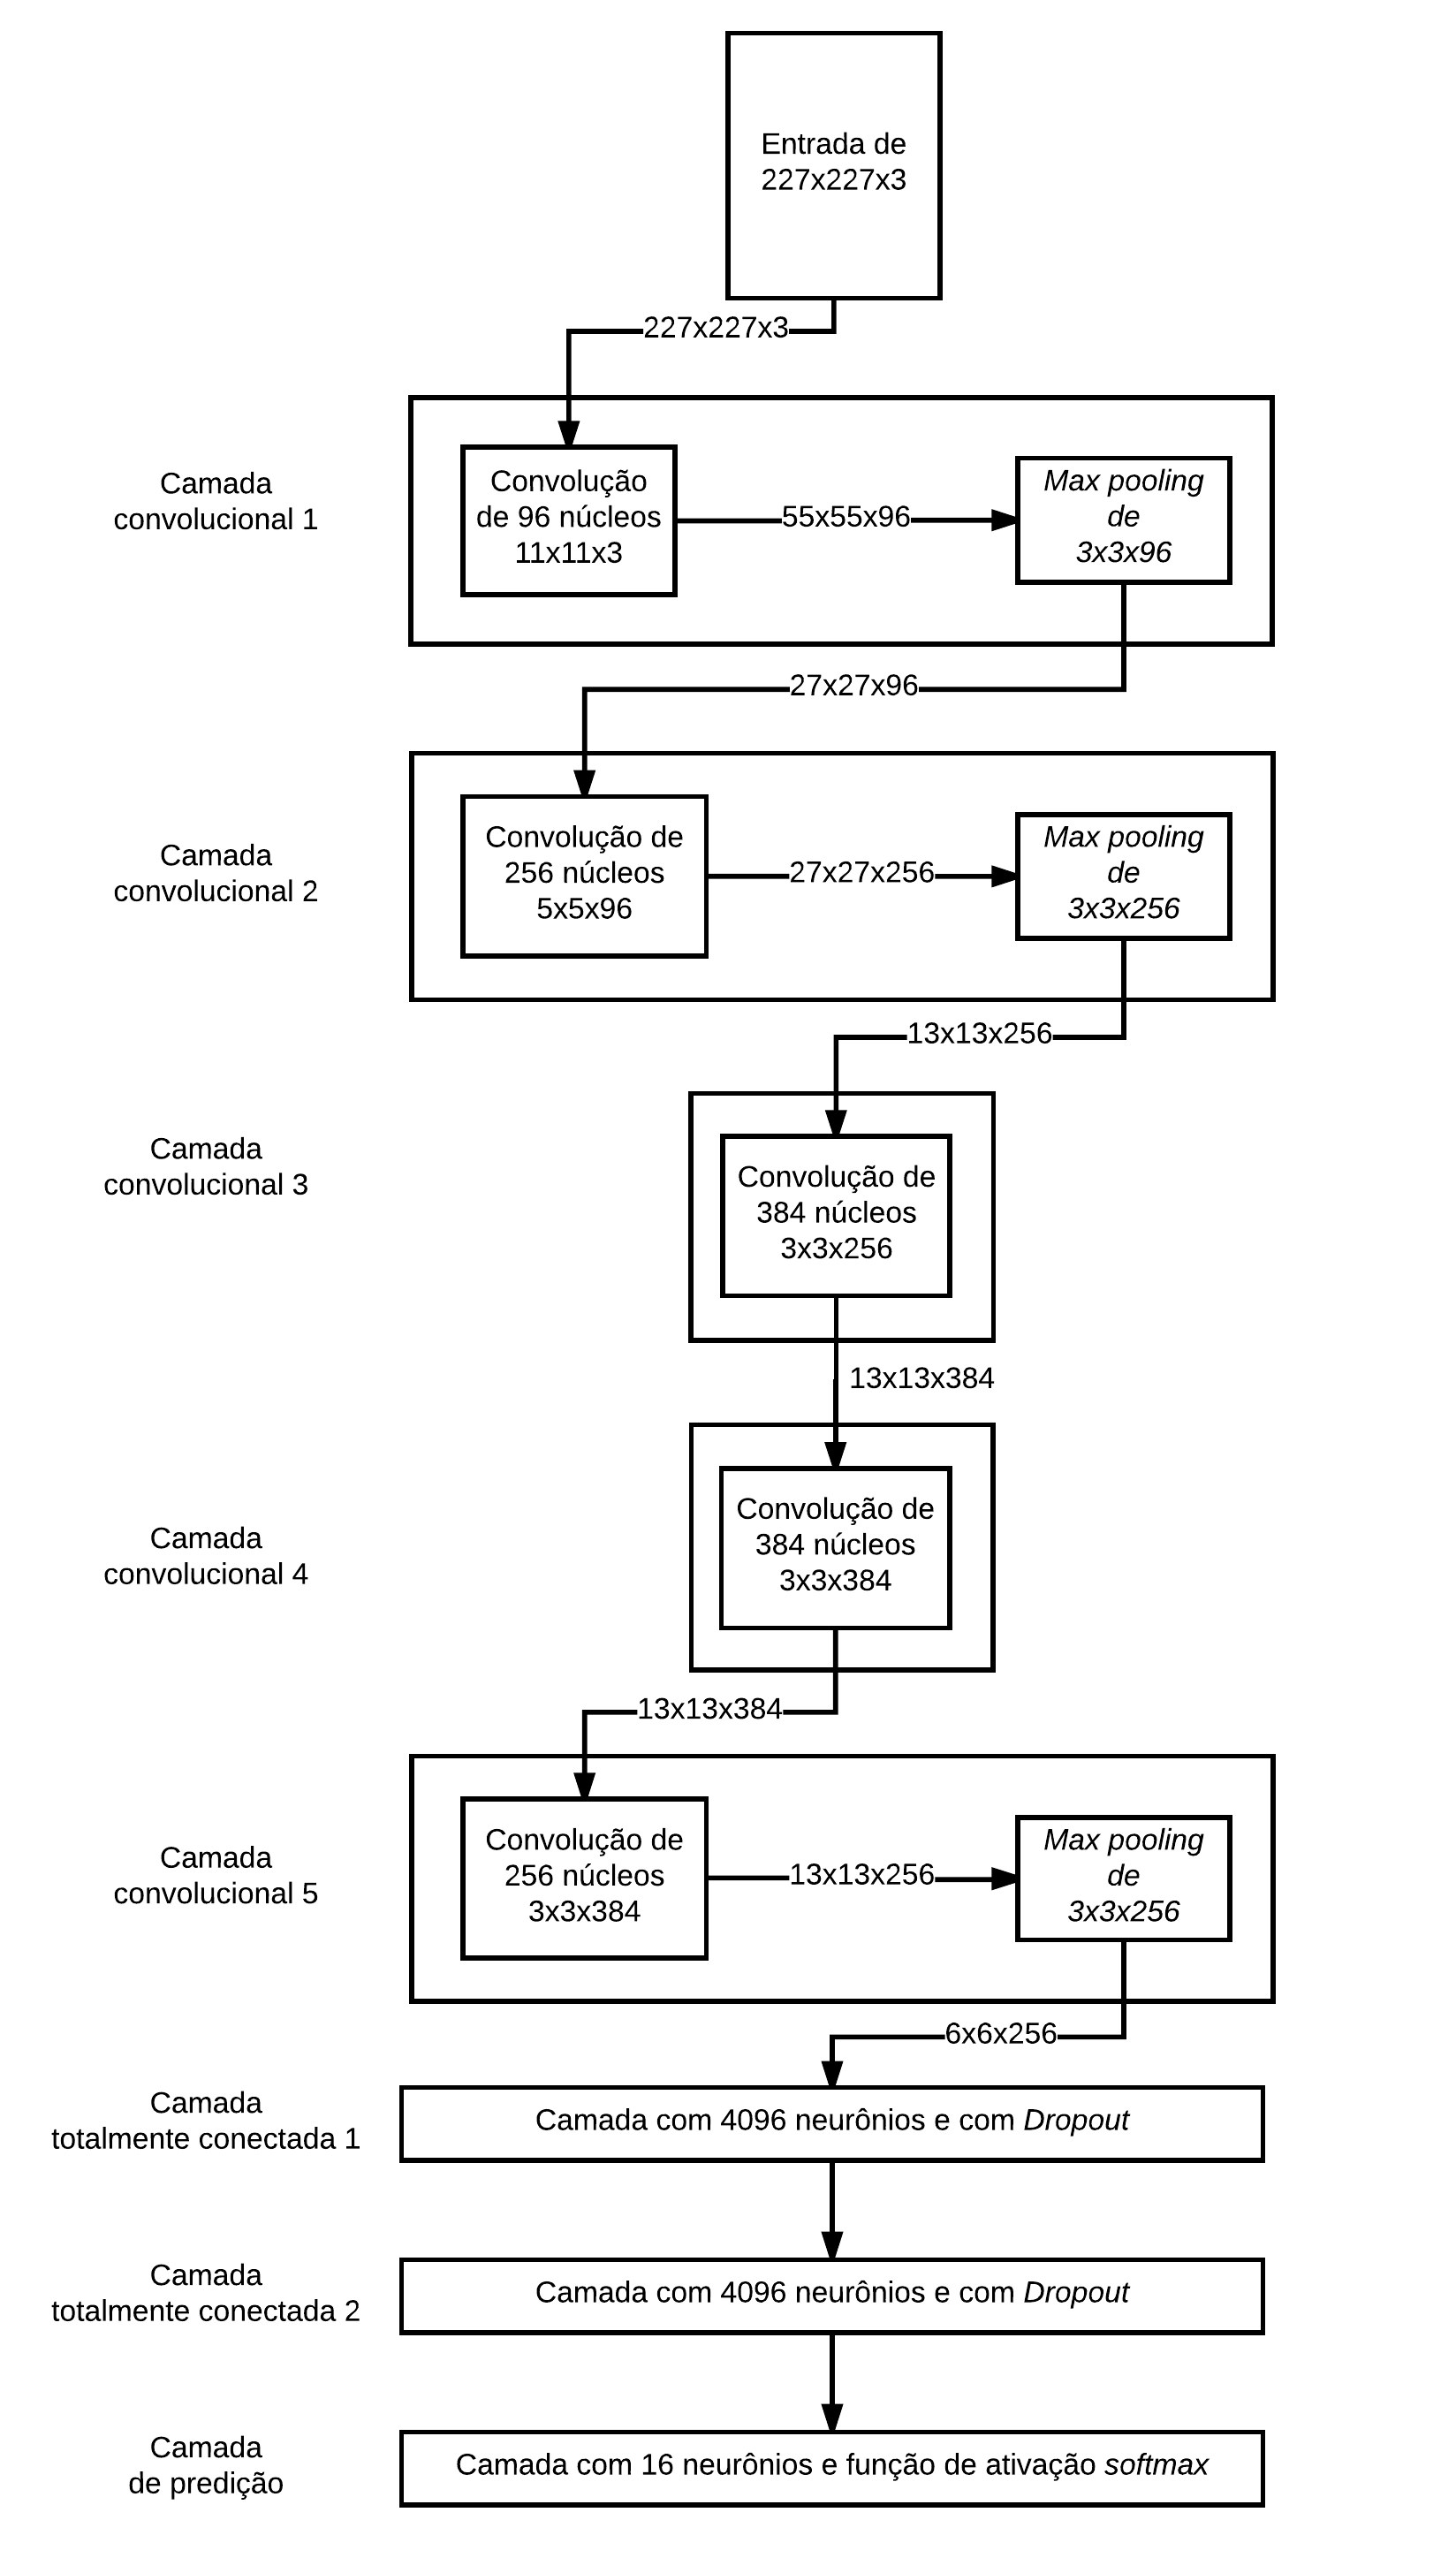
\includegraphics[width=350pt]{dados/figuras/dia_rede}
  \label{fig:arqrede}
\end{figure}

\par Foi utilizado o \textit{framework} \textit{Keras} \cite{chollet2015keras} para implementar a rede neural. \textit{Keras} é um \textit{framework} em \textit{python} para execução de redes neurais utilizando \textit{GPU}(\textit{Graphics Processing Unit}). Com o \textit{keras} é possível configurar em alto nível uma rede neural, abstraindo a complexidade da descrição e implementação das rotinas de execução das camadas. Como exemplo de implementação, temos a \autoref{fig:conv_keras}, contendo a codificação da primeira e segunda camada da rede neural proposta. Neste projeto o \textit{keras} está sendo utilizado com o \textit{back end Theano} \cite{2016arXiv160502688full} para a geração de código em \textit{Cuda}, linguagem que compila codigo para ser executado em GPU.
\begin{figure}[H]
  \centering
  \caption{Trecho de código com implementação utilizando o \textit{framework} \textit{keras} das duas primeiras camadas convolucionais da rede neural, contendo a definição da entrada e as implementações das camadas de transição entre as camadas de convolução um e dois.}
  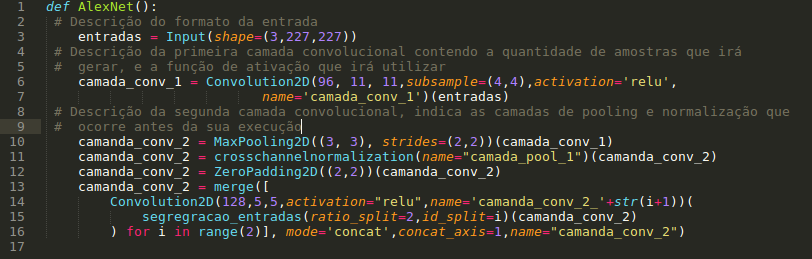
\includegraphics[width=400pt]{dados/figuras/exemplo_keras}
  \label{fig:conv_keras}
\end{figure}


\section{Melhorias para a rede neural proposta}

Melhorias no desempenho de redes neurais podem ser aplicadas em diversas etapas do processo de aprendizado e classificação. O aumento da base de treino, a definição de quais camadas devem ser treinadas em determinadas épocas, a inicialização dos pesos da rede neural com valores de uma rede treinada com uma quantidade maior de amostras e o aprimoramento dos parâmetros de configuração da rede, são métodos que podem ser utilizados para aprimorar seu desempenho de classificação.

\par Neste projeto foram aplicadas técnicas para a melhorar a classificação, sendo elas
%técnicas o ajuste empírico da taxa de descarte de neurônios nas camadas totalmente conectadas,
o aumento dos dados na base de treino e a inicialização dos pesos da rede neural com pesos de uma rede já treinada. %Essas técnicas são descritas mais detalhadamente nas seções a seguir.

\subsection{\textit{Data augmentation}}
Uma técnica que vem sendo muito utilizada no para a redução do \textit{overfitting} na fase de treino de uma rede neural é a \textit{data augmentation} \cite{cui2015data}. 
Os dados da base são ligeiramente modificados para se obter o aumento na quantidade de amostras.
Essas mudanças podem ser inversões nos eixos, pequenas rotações, aproximações em certas partes das imagens ou até a aplicação da imagem em escala cinza.
Essa técnica tem o propósito de aumentar a quantidade de amostras em que serão realizados os treinos, buscando evitar um \textit{overfitting} \cite{imaginetArticle}.
\par Nesse projeto foi utilizada a técnica de \textit{data augmentation} aplicando inversão no eixo $y$, realizando um zoom de aproximação ou distanciamento de até 20\% e aplicado uma taxa de inclinação de até 0,2 radianos. As amostras foram geradas com a combinação das transformações possíveis informadas, criando nove imagens a partir de cada imagem de treino, como representado na \autoref{fig:data_augmentation}. Essas imagens foram geradas durante a execução do treino da rede e foram armazenadas em memória.

\begin{figure}[H]
  \centering
  \caption{Imagem representado a técnica de \textit{data augmentation} aplicada na base de treino. A imagem no centro é a original, e as outras são possíveis modificações aplicadas sobre ela, como a inversão do eixo $y$ e o aumento e diminuição do \textit{zoom}.}
  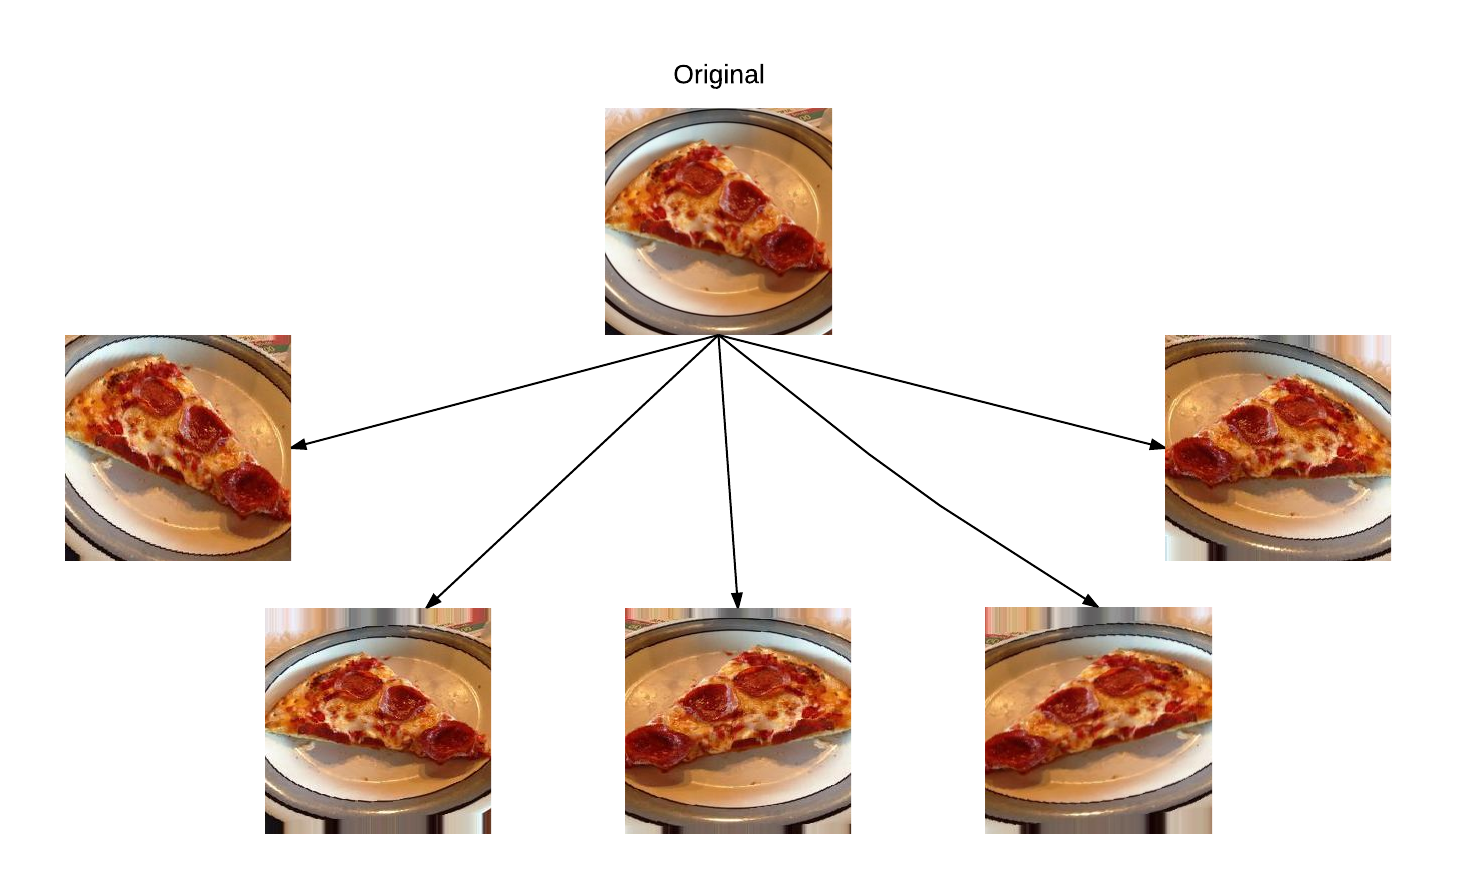
\includegraphics[width=500pt]{dados/figuras/data_augmentation}
  \label{fig:data_augmentation}
\end{figure}

\subsection{Inicialização dos pesos}
Uma rede neural treinada do início ao fim tem seus pesos inicializados de maneira aleatória e, conforme vai realizando suas predições, os pesos são corrigidos para melhorar o poder de classificação. A inicialização dos pesos da rede neural com valores obtidos a partir de uma rede treinada vem sendo utilizada como maneira de melhorar a classificação \cite{Girshick_2014_CVPR}. Geralmente os pesos vêm de redes que treinaram uma quantidade muito grande de dados, conseguindo de certa forma transferir o aprendizado obtido para a rede que está inicializando os pesos. Nesse projeto foi realizada a inicialização dos pesos da rede neural utilizando os pesos obtidos no treinamento da rede desenvolvida por \citeonline{imaginetArticle} para melhorar o desempenho da rede neural proposta.

% \subsection{Congelamento de camadas}

% \par O aprimoramento da rede neural convolucional pode ser feito por meio da utilização de parâmetros já treinados da rede neural, \cite{Girshick_2014_CVPR} descreve esse método como um pré-treino da rede, a preparando para a sua real tarefa. Podendo assim utilizar os pesos treinados em \cite{imaginetArticle} para um aperfeiçoamento da rede.
% \par Outro método utilizado para a melhora do resultado e redução do \textit{overfit}(quando um classificador não produz resultados bons de classificação para entradas diferentes das contidas na base de dados) é o de poda na rede \cite{NIPS2015_5784}. Onde os pesos de conexão podem ser agrupados por meio de \textit{hash} identificando parâmetros similares entre eles, tendo assim um parâmetro para cada grupo de peso.
% \par Uma técnica utilizada para o aumento da base de dados é o \textit{data aumentation}, onde os dados da base são ligeiramente modificados, para obter um crescimento da base. Essa técnica é aplica para reduzir o \textit{overfit} e aumentar a base de teste. Essas mudanças nas imagens podem ser inversões das imagens, pequenas rotações ou aproximações em certas partes das imagens.


%Melhorias no desempenho de redes neurais podem ser aplicadas em diversas etapas do processo de aprendizado e classificação. O aumento da base de treino por meio de técnicas de \textit{data augmentation} \cite{imaginetArticle}\cite{cui2015data}, definir quais camadas serão treinadas em determinadas épocas utilizando a técnica conhecida como \textit{layer-wise} \cite{tajbakhsh2016convolutional}, a inicialização dos pesos da rede com valores de uma rede treinada com uma quantidade maior de amostras técnica conhecida como \textit{transfer learning} (em português, transferência de aprendizagem)\cite{Girshick_2014_CVPR}, são métodos  